\documentclass[11pt]{article}
\usepackage[utf8]{inputenc}
\usepackage[english]{babel}
\usepackage[font=small,labelfont=bf]{caption}
\usepackage{geometry}
\usepackage[sort&compress, numbers, super]{natbib}
\usepackage{pxfonts}
\usepackage{graphicx}
\usepackage{setspace}
\usepackage{hyperref}
\usepackage{lineno}

\newcommand{\argmax}{\mathop{\mathrm{argmax}}\limits}

\newcommand{\dynamicsRandom}{S1}
\newcommand{\dynamicsAdaptive}{S2}
\newcommand{\fingerprintsRandom}{S3}
\newcommand{\fingerprintsAdaptive}{S4}
\newcommand{\recallInit}{S5}

\doublespacing
\linenumbers

\title{Carryover effects in free recall reveal how prior experiences influence memories of new experiences}
\author{Jeremy R. Manning\textsuperscript{1, *}, Andrew C. Heusser\textsuperscript{1, 2}, Kirsten Ziman\textsuperscript{1, 3},\\Emily Whitaker\textsuperscript{1}, and Paxton C. Fitzpatrick\textsuperscript{1}\\\textsuperscript{1}Dartmouth College\\\textsuperscript{2}Akili Interactive\\\textsuperscript{3}Princeton University\\\textsuperscript{*}Corresponding author: jeremy.r.manning@dartmouth.edu}

\date{}

\begin{document}
\maketitle

\begin{abstract} We perceive, interpet, and remember ongoing experiences
through the lens of our prior experiences. Inferring that we are one type of
situation versus another can lead us to interpret the same physical experience
differently. In turn, this can affect how we focus our attention, form
expectations of what will happen next, remember what is happening now, draw on
our prior related experiences, and so on. To study these phenomena, we asked
participants to perform simple word list learning tasks. Across different
experimental conditions, we held the set of to-be-learned words constant, but
we manipulated the orders in which the words were studied. We found that these
order manipulations affected not only how the participants recalled the ordered
lists, but also how they recalled later randomly ordered lists. Our work shows
how structure in our ongoing experiences can exert influence on how we remember
unrelated subsequent experiences. \end{abstract}


\section*{Introduction}

% the role of context and prior experience in memory 

Experience is subjective: different people who encounter identical physical
experiences can take away very different meanings and memories. One reason is
that our subjective experiences in the moment are shaped in part the
idiosyncratic prior experiences, memories, goals, thoughts, expectations, and
emotions that we bring with us into the present moment. These factors
collectively define a \textit{context} for our experiences~\citep{Mann20}. %
situation models: forming expectations, predicting ambiguous future experiences
The contexts we encounter help us to construct \textit{situation
models}~\citep{RangRitc12, MannEtal15} or \textit{schemas}~\citep{MasiEtal22,
BaldEtal18} that describe how experiences are likely to unfold based on our
prior experiences with similar contextual cues. For example, when we enter a
sit-down restaurant, we might expect to be seated at a table, given a menu, and
served food. Priming someone to expect a particular situation or context can
also influence how they resolve potentail ambiguities in their ongoing
experiences, including ambiguous movies and narratives~\citep{YeshEtal17}.

% gap between "classic" free recall tasks and naturalistic (or real-world)
% memory tasks 

Our understanding of how we form situation models and schemas, and how they
interact with our subjective experiences and memories, is constrained in part
by substantial differences in how we study these processes. Situation models
and schemas are most often studied using ``naturalistic'' stimuli such as
narratives and movies~\citep{ZwaaEtal95,ZwaaRadv98, NastEtal20}. In contrast,
our understanding of how we organize our memories has been most widely studied
using more traditional paradigms like free recall of random word
lists~\citep{Kaha12}. In free recall, participants study lists of items and are
instructed to recall the items in any order they choose. The orders in which
words come to mind can provide insights into how participants have organized
their memories of the studied words. Because random word lists are unstructured
by design, it is not clear if or how non-trivial situation models might apply
to these stimuli. Nevertheless, there are \textit{some} commonalities between
memory for word lists and memory for real-world experiences.

Like remembering real-world experiences, remembering words on a studied list
requires distinguishing the current list from the rest of one's experience. To
model this fundamental memory capability, cognitive scientists have posited the
existence of a special representation, called \emph{context}, that is
associated with each list. According to early
theories~\citep[e.g.][]{Este55a,AndeBowe72} context representations are
composed of many features which fluctuate from moment to moment, slowly
drifting through a multidimensional feature space. During recall, this
representation forms part of the retrieval cue, enabling us to distinguish list
items from non-list items. Understanding the role of context in memory
processes is particularly important in self-cued memory tasks, such as
\textit{free recall}, where the retrieval cue is ``context'' itself.

Over the past half-century, context-based models have enjoyed impressive
success at explaining many stereotyped behaviors observed during free recall
and other list-learning tasks~\citep{Este55a, RaaiShif80, GlenEtal83,
HowaKaha02a, SiroEtal05, KimbEtal07, PolyKaha08, PolyEtalTulv, SedeEtal08,
PolyEtal09, ShanHowa12}. These phenomena include the well-known recency and
primacy effects (superior recall of items from the end and, to a lesser extent,
from the beginning of the study list), as well as semantic and temporal
clustering effects~\citep{KahaEtal08}. The contiguity effect is an example of
temporal clustering, which is perhaps the dominant form of organization in free
recall. This effect can be seen in the tendency for people to successively
recall items that occupied neighboring positions in the study list. For
example, if a list contained the sub-sequence \textsc{``absence hollow pupil''}
and the participant recalls the word \textsc{``hollow''}, it is far more likely
that the next response will be either \textsc{``pupil''} or
\textsc{``absence''} than some other list item~\citep{Kaha96}. In addition,
there is a strong forward bias in the contiguity effect: subjects make forward
transitions (i.e., \textsc{``hollow''} followed by \textsc{``pupil''}) about
twice as often as they make backward transitions, despite an overall tendency
to begin recall at the end of the list. There are also striking effects of
semantic clustering~\citep{RomnEtal93, Bous53, BousEtal54, JenkRuss52,
MannKaha12}, whereby the recall of a given item is more likely to be followed
by recall of a similar or related item than a dissimilar or unrelated one. In
general, people organize memories for words along a wide variety of stimulus
dimensions. As captured by models like the \textit{Context Maintenance and
Retrieval Model}~\citep{PolyEtal09}, the stimulus features associated with each
word (e.g.\ the word's meaning, font size, font color, location on the screen,
size of the object the word represents, etc.) are incorporated into the
participant's mental context representation~\citep{SmitVela01, MannEtal15,
Mann20, MannEtal11, MannEtal12}. During a memory test, any of these features
may serve as a memory cue, which in turn leads the participant to recall in
succession words that share stimulus features.

% link clustering to schemas...

A key mystery is whether the sorts of situation models and schemas that people
use to organize their memories of real-world experiences might map onto the
clustering effects that reflect how people organize their memories for word
lists. On one hand, situation models and clustering effects both reflect
statistical regularities in ongoing experience. Our memory systems exploit
these regularities when generating inferences about the unobserved past and
yet-to-be-experienced future~\citep{XuEtal22, SchaTurk15, RangRitc12,
BoweEtal79, MomeEtal17}. On the other hand, the rich structure of real-world
experiences and other naturalistic stimuli that enable people to form deep and meaningful
situation models and schemas have no obvious analog in simple word lists.  Often lists
in free recall studies are explicitly \textit{designed} to be devoid of exploitable
temporal structure, for example by sorting the words in a random order~\citep{Kaha12}.

% feature-rich free recall, basic manipulation conditions, preview of findings
We designed an experimental paradigm to explore how people organize their
memories for simple stimuli (word lists) whose temporal properties change
across different ``situations,'' analogous to how the content of real-world
experiences change across different real-world situations. We asked
participants to study and freely recall a series of word lists
(Fig.~\ref{fig:exp}). Across the different conditions in the experiment, we
varied the lists' presentation orders in different ways across lists. The
studied items (words) were designed to vary along three general dimensions:
semantic (word \textit{category}, and physical \textit{size} of the referent),
lexicographic (word \textit{length} and \textit{first letter}), and visual
(font \textit{color} and the onscreen \textit{location} of each word). In our
main manipulation conditions, we asked participants to study and recall eight
lists whose items were sorted by a target feature (e.g., word category). Next,
we asked them to study and recall an additional eight lists whose items had the
same features, but that were sorted in a random temporal order. We were
interested in how these order manipulations affected participants' recall
behaviors on early (sorted) lists, as well as how order manipulations on early
lists affected recall behaviors on later (unsorted) lists. We used a series of
control conditions as a baseline; in these control conditions all of the lists
were sorted randomly, but we manipulated the presence or absence of the visual
features. Finally, in an \textit{adaptive} experimental condition we used
participants' recall behaviors on early lists to manipulate, in real-time, the
presentation orders of subsequent lists. In this adaptive condition, we sought
to identify potential commonalities within and across participants in how
people organized their memories and how those organizational tendancies affect
overall performance.

\begin{figure} 
    \begin{center}
        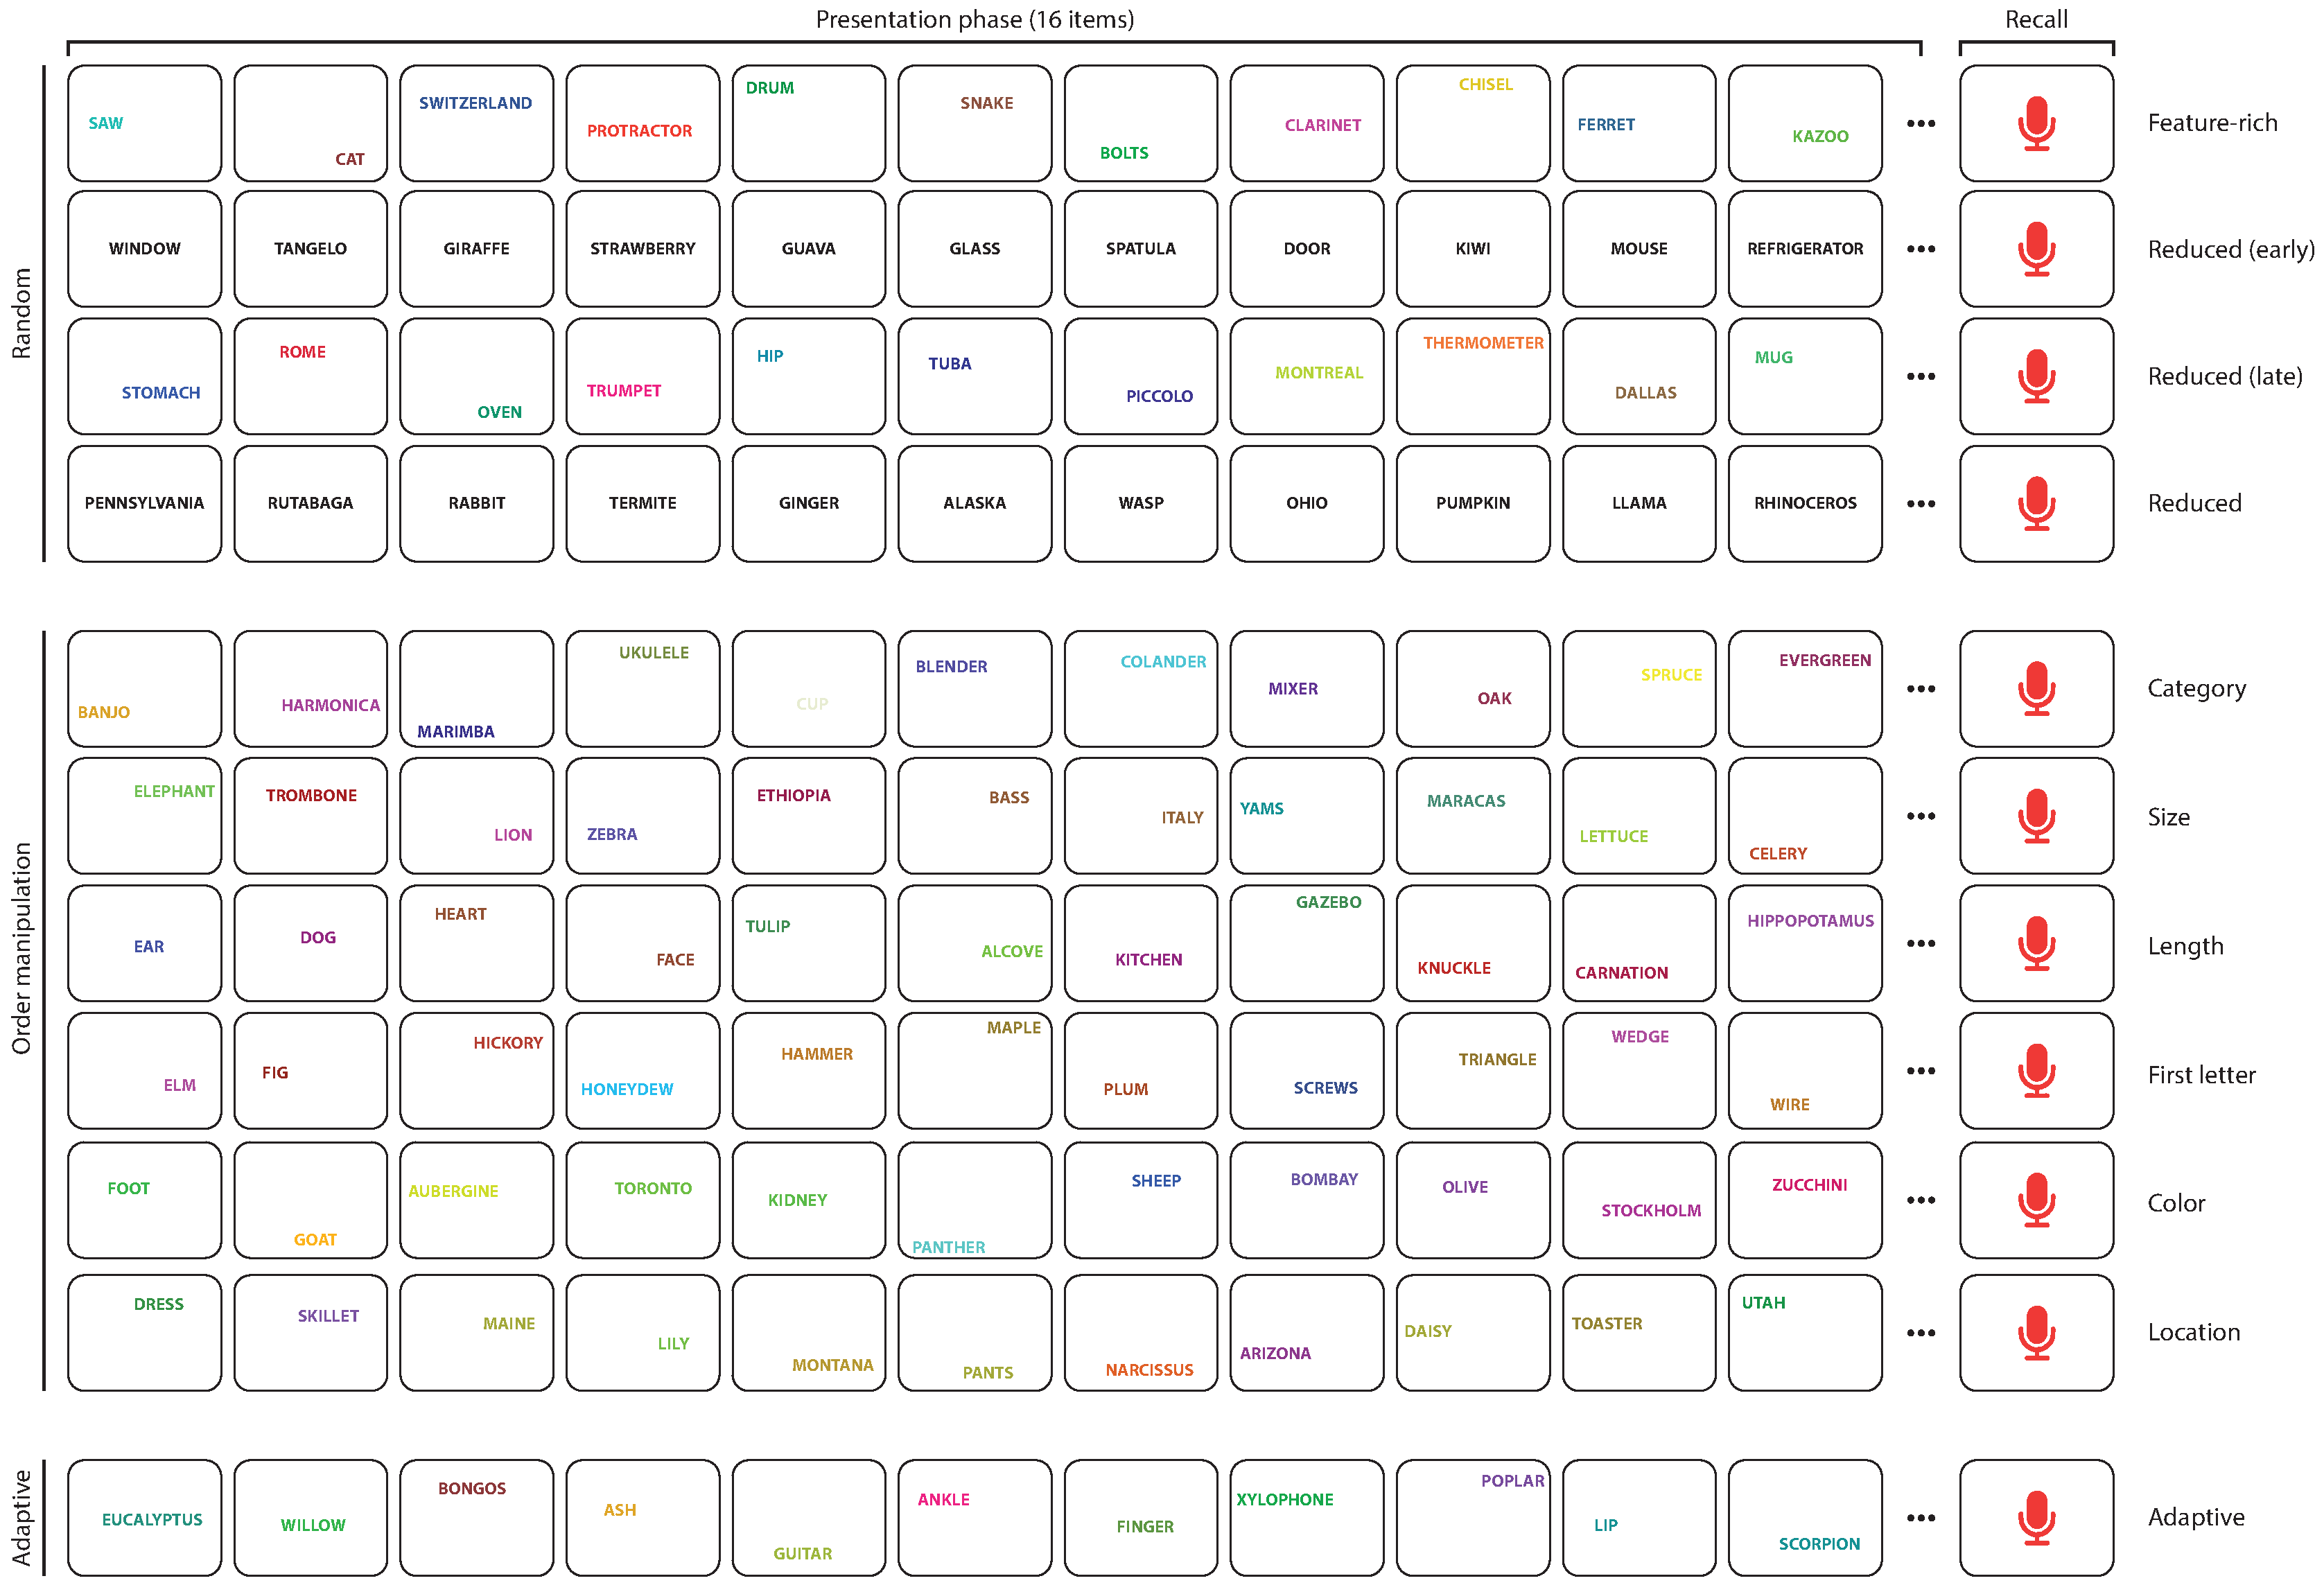
\includegraphics[width=0.4 \textwidth]{figures/FRFR} \end{center} \vspace{-16pt}
        
        \caption{\textbf{Feature-rich free recall.} After studying lists
comprised of words that vary along several feature dimensions, participants
verbally recall words in any order (microphone icon).} 

    \label{fig:exp}
\end{figure}







\section*{Results}

\begin{figure}[tp] \centering
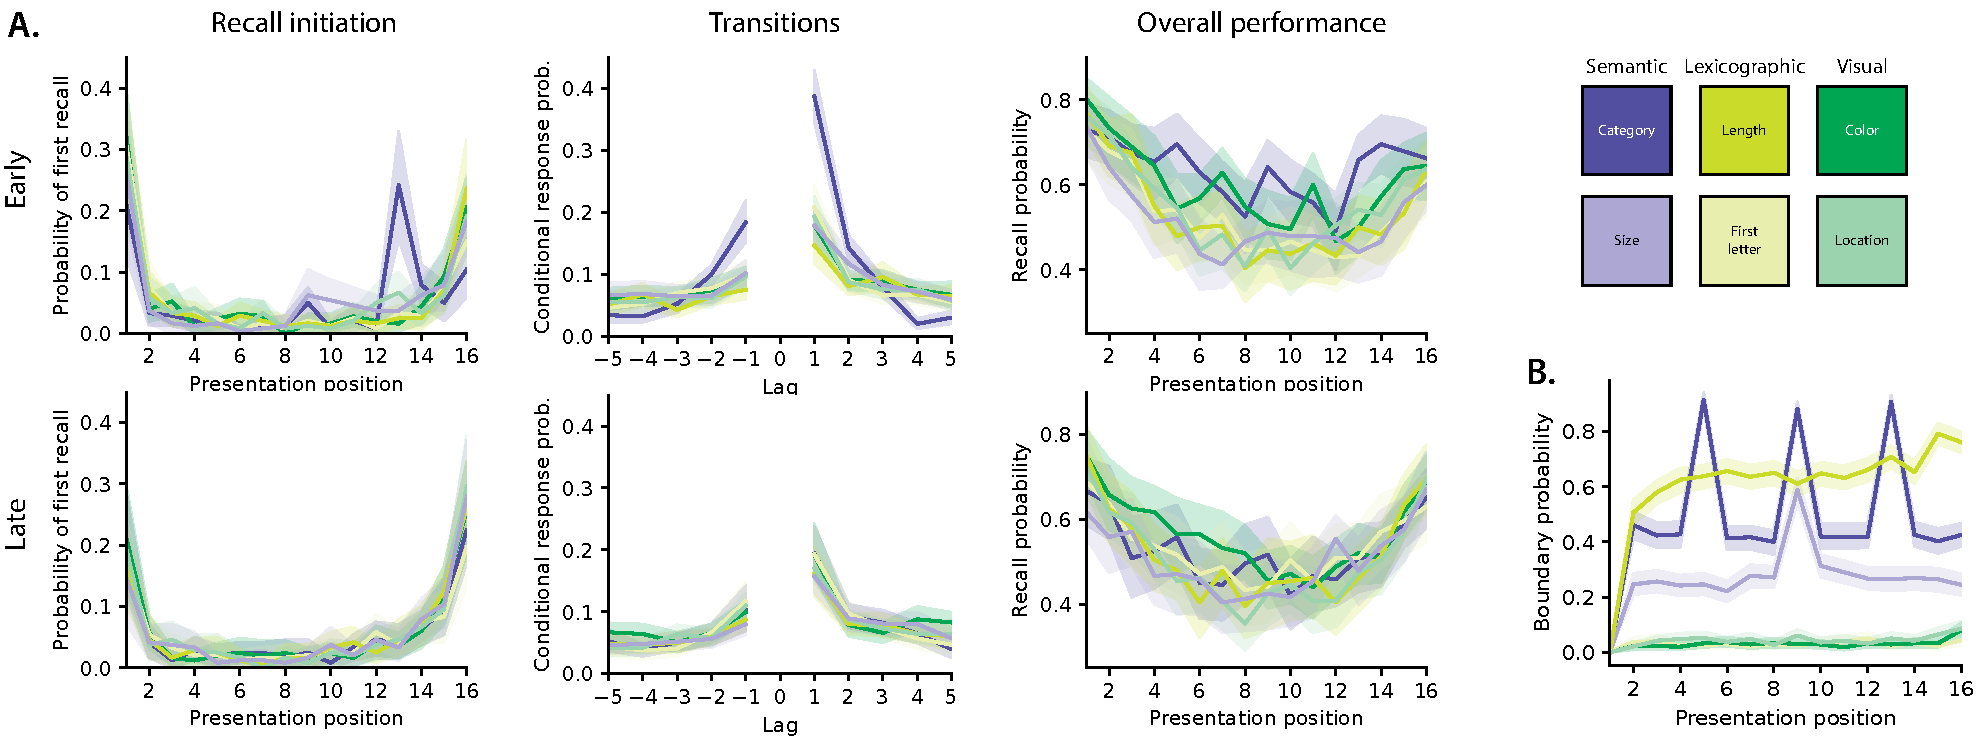
\includegraphics[width=\textwidth]{figures/recall_dynamics}

\caption{\textbf{Recall dynamics in feature rich free recall (order
manipulation conditions).} \textbf{Left panels.} The probabilities of
initiating recall with each word are plotted as a function of presentation
position. \textbf{Middle panels.} The conditional probabilities of recalling
each word are plotted as a function of the relative position (Lag) to the words
recalled just-prior. \textbf{Right panels.} The overall probabilities of
recalling each word are plotted as a function of presentation position.
\textbf{All panels.} Error ribbons denote bootstrap-estimated 95\% confidence
intervals (calculated across participants). Top panels display the recall
dynamics for early (order manipulation) lists in each condition (color). Bottom
panels display the recall dynamics for late (randomly ordered) lists.  See
Figures~\dynamicsRandom~and~\dynamicsAdaptive~for analogous plots for the random (control) and adaptive conditions.}

    \label{fig:recall-dynamics}
\end{figure}

% figure: clustering effects
\begin{figure}[tp] \centering
    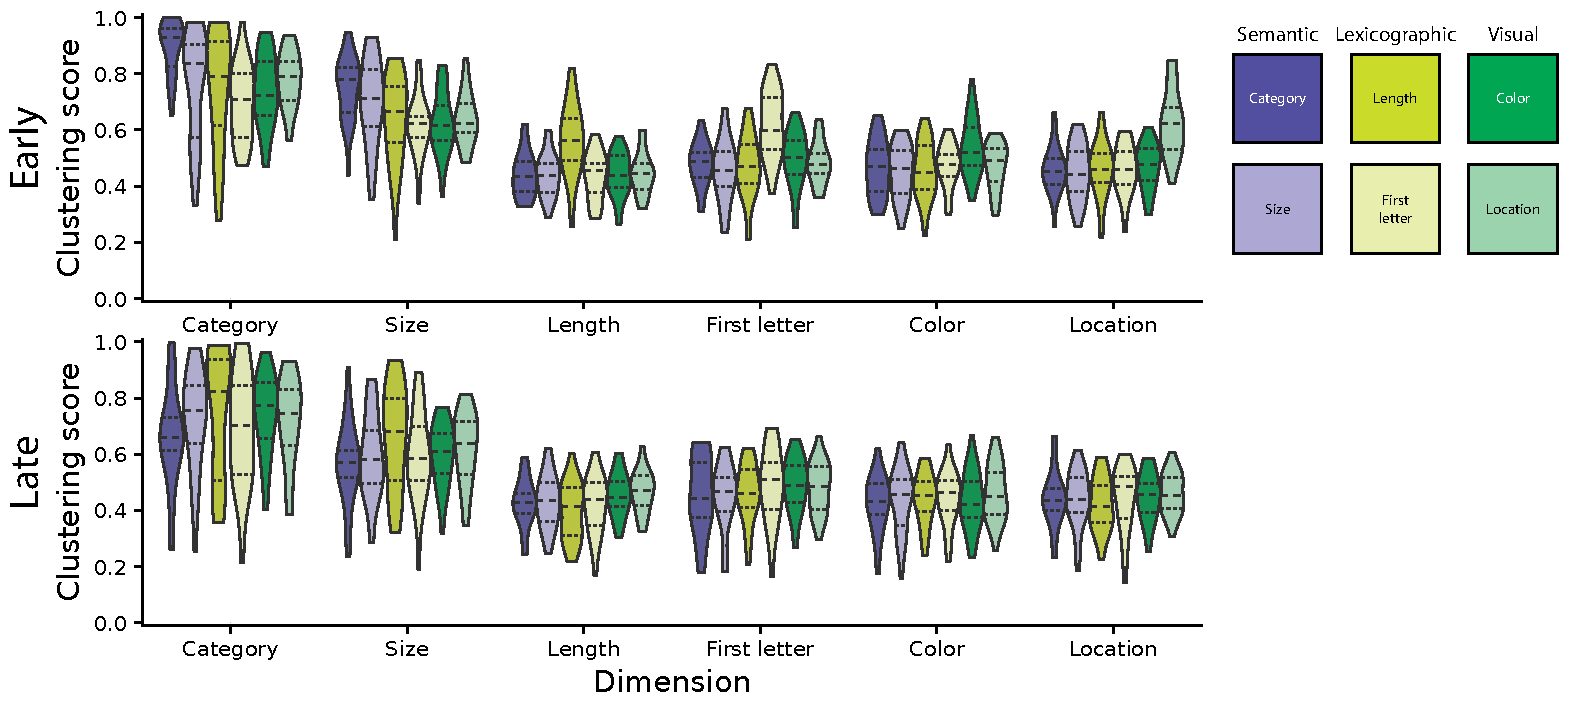
\includegraphics[width=\textwidth]{figures/fingerprints}
    
    \caption{\textbf{Memory ``fingerprints.'' (order manipulation conditions).}
    The across-participant distributions of clustering scores for each feature
    type ($x$-coordinate) are displayed for each experimental condition
    (color), separately for order manipulation (early, top) and randomly
    ordered (late, bottom) lists. See
    Figures~\fingerprintsRandom~and~\fingerprintsAdaptive~for analogous plots
    for the random (control) and adaptive conditions.}
        \label{fig:fingerprints}
    \end{figure}


% figure: recall initiation
Figure~\recallInit.

% figure: feature clustering vs. accuracy, feature clustering vs. temporal clustering

% figure: fingerprint trajectories

% figure: carryover effects: clustering early vs. clustering late

% figure: clustering carryover vs. accuracy difference

% figure: clustering carryover vs. temporal clustering differences

\section*{Discussion}

% recap

% connections to prior work: context effects, priming, situation models

% implications for adaptive learning, education and training


\section*{Materials and methods}
\subsection*{Participants}

\subsection*{Experimental design}

\subsection*{Analysis}

\bibliographystyle{apa}
\bibliography{CDL-bibliography/cdl}
\end{document}
